\documentclass[usenames,dvipsnames,pdf]{beamer}

\usepackage{textcomp}
\usepackage{pifont}
\usepackage[utf8]{inputenc}
\usepackage{amsfonts}
\usepackage{amstext}
\usepackage{amsmath}
\usepackage{fancyhdr}
\usepackage{amsthm}
\usepackage{epsfig}
\usepackage{graphicx}
\usepackage{multicol}
\usepackage{cite}
\usepackage{natbib}
\usepackage{adjustbox}
\usepackage{bussproofs}
\usepackage{stmaryrd}
\usepackage[tableaux]{prooftrees}
\usepackage{qtree}
\usepackage{mathtools}
\usepackage{scalerel,stackengine}
\usepackage[all]{xy}
% \usetikzlibrary{automata, positioning, shapes, arrows}
% \usepackage[dvipsnames]{xcolor}

\usetheme{CambridgeUS}

%\useoutertheme{miniframes} % Alternatively: miniframes, infolines, split
%\useinnertheme{circles}

%\definecolor{UBCblue}{rgb}{0.04706, 0.13725, 0.26667} % UBC Blue (primary)

% \usecolortheme[named=UBCblue]{structure}
% \usecolortheme[named=RoyalBlue]{structure}
\usecolortheme{seahorse}

% \usecolortheme{beaver}
%\setbeamercolor{spruce}{fg=cyan!90!black}

%\setbeamertemplate{itemize item}{\color{teal}$\blacktriangleright$}
%\setbeamertemplate{itemize subitem}{\color{teal}$\blacktriangleright$}

\renewcommand{\phi}{\varphi}

\graphicspath{ {./images/} }


% \newcommand{\newState}[4]{\node[state,#3](#1)[#4]{#2};}
% \newcommand{\newTransition}[4]{\path[->] (#1) edge [#4] node {#3} (#2);} 
\renewcommand*\linenumberstyle[1]{(#1)}
\def\apeqA{\SavedStyle\sim}
\def\apeq{\setstackgap{L}{\dimexpr.5pt+1.5\LMpt}\ensurestackMath{%
  \ThisStyle{\mathrel{\Centerstack{{\apeqA} {\apeqA}}}}}}

\def\dis{\displaystyle}

\def\QQ{\mathbb Q}
\def\ZZ{\mathbb Z}
\def\RR{\mathbb R}
\def\CC{\mathbb C}
\def\FF{\mathbb F}
\def\NN{\mathbb N}
\def\AA{\mathbb A}
\def\II{\mathbb I}

\def\Cc{\mathcal C}
\def\Dd{\mathcal D}
\def\Pp{\mathcal P}

\def\Af{\mathfrak A}
\def\Bf{\mathfrak B}
\def\Cf{\mathfrak C}
\def\Df{\mathfrak D}
\def\Ef{\mathfrak E}
\def\Ff{\mathfrak F}
\def\Gf{\mathfrak G}
\def\Hf{\mathfrak H}
  
% define 2x2 matrix:
\newcommand\twodmatrix[4]{ \ensuremath{ \left( 
	\begin{array}{cc}
		#1 & #2  \\
		#3 & #4 
	\end{array}  
	\right) } }
  

%%%%%%%%%%%%%%%%%%%%%%%%%%%%%%%%%%%%%%%%%%%%%
\setbeamerfont{footnote}{size=\tiny}

\DeclareMathSymbol{:}{\mathord}{operators}{"3A}

\mode<presentation>{}
%% preamble
\title{A sequence-to-sequence approach for document-level relation extraction}
\author{John Giorgi, Gary D. Bader, Bo Wang}
\begin{document}
	%% title frame
	\begin{frame}
		\titlepage
	\end{frame}


        \section{Overview}

        \begin{frame}{Introduction}
          \begin{itemize}
          \item
            Novel end-to-end joint learning approach for inter-sentence relation extraction.\footnote{Document-level is a stretch, due to encoder limit of 512 tokens they did paragraphs.}
          \item
            Utilizes sequence to sequence architecture.
          \item
            Representation for coreferent entities and $n$-ary relations (\textit{Linearization schema}).
          \item
            Can also handle discontinuous (disjoint) and nested entity spans.  
          \end{itemize}
        \end{frame}

        \begin{frame}{Introduction}
          \begin{itemize}
          \item
            New benchmarks for end-to-end results over some biomedical datasets.
          \item
            SOTA for RE with gold entities on two biomedical datasets (DGM, GDA).
          \item
            Competitive results against more complex architectures for datasets
            with established end-to-end and gold entity RE results.
          \end{itemize}
          
        \end{frame}

        \begin{frame}{Defining Terms}
          End-to-end RE:
          \begin{itemize}
          \item
            Relation extraction depends on entities.
          \item
            Pipeline methods (current standard),
            use one or more models for NER,
            and one or more models for RE over discovered entities.
          \item
            End-to-end approaches use one model
            (possibly with a classification head)
            to discover the relations,
            relying on internal representations to jointly extract
            and implicitly coordinate entity and relation information.
          \end{itemize}

          \textbf{NB:}  The authors use \textit{pipeline} to refer to the RE component.
          In NER/RE practice, pipeline usually refers to the whole system, NER included.  
        \end{frame}

        \begin{frame}{Defining Terms}
          Coreference:
          \begin{itemize}
          \item
            The same entity may have one or more mentions in a given text unit (type vs. token).
          \item
            If a relation holds between two entites, how to reflect this for each entity's mentions?
          \end{itemize}
        \end{frame}

        \begin{frame}{Defining Terms}
          Sequence to sequence (seq2seq):
          \begin{itemize}
          \item
            Encoder to decoder.
          \item
            Encoder maps each input token to a contextual representation.
          \item
            Decoder maps each encoder token output and prior context to an output token.
          \item
            Sequence cross-entropy loss used in training.
          \end{itemize}
        \end{frame}
        
        \begin{frame}{Motivation}
          \begin{itemize}
          \item
            Lots of entity and relation information at the document and cross document level.
          \item
            Generalizing sentential pipeline methods (the current standard)
            for inter-sentential RE is involved.\footnote{e.g. our NER/RE system for radiotherapy.}
          \item
            Lots of information takes the form of $n$-ary relations, not always easy to reconstruct this from binary relations.
          \item
            Handling discontinuous/disjoint and nested entity spans is helpful and not entirely solved.
          \end{itemize}
        \end{frame}
        
        \section{Method}


        \begin{frame}{Datasets}
          \begin{itemize}
          \item \textbf{CDR}


            Chemical-induced disease (CID) relations, binary relations.   
          \item \textbf{GDA}


            Gene-disease associations, binary relations.  
          \item \textbf{DGM}

            Drug-gene-mutations, ternary relations.   
          \item \textbf{DocRED}
            General domain, binary relations.
            
          \end{itemize}
        \end{frame}

        \begin{frame}{Datasets}
          \begin{figure}
            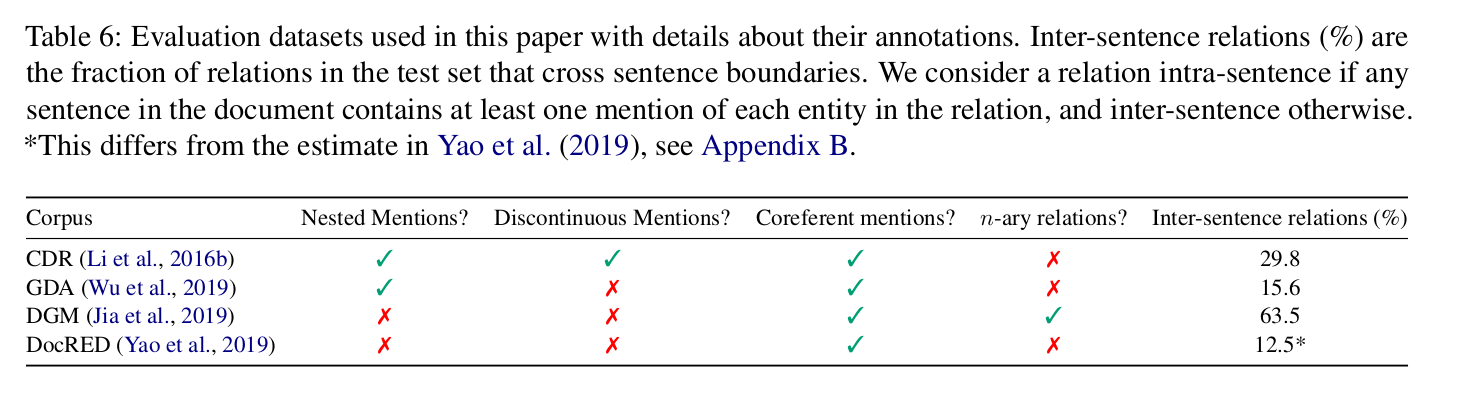
\includegraphics[width=1.0\textwidth,height=1.0\textheight,keepaspectratio]{datasetinfo} 
          \end{figure}
        \end{frame}
       
        
        \begin{frame}{Linearization Schema}
          \begin{figure}
          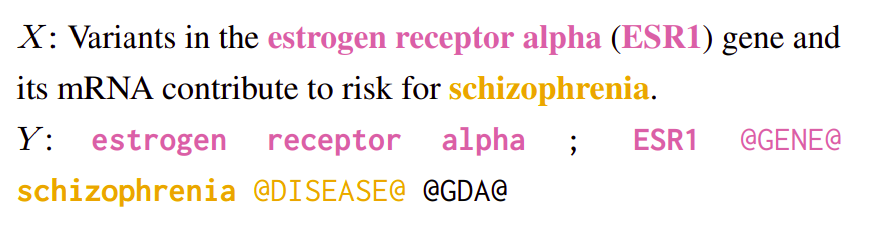
\includegraphics[width=0.7\textwidth,height=0.7\textheight,keepaspectratio]{linearization} 
          \end{figure}
          Full schema:

          
          \begin{adjustbox}{varwidth=\linewidth}%,scale=0.7}
            %% \begin{framed}
            %\centering
            \small\text{$<\textit{entity mention}_{1,1}>$ ; ... ; $<\textit{entity mention}_{1,n}>$ $@<\textit{entity type}_1 > @ \dots$}


            \small\text{$<\textit{entity mention}_{m,1}>$ ; ... ; $<\textit{entity mention}_{m,k}>$ $@<\textit{entity type}_m > @$}


            \small\text{$@ <\textit{relation type}> @$}
            \end{adjustbox}
        \end{frame}

        
        \begin{frame}{Model Structure}
          \begin{itemize}
          \item
            Seq2seq architectre.
          \item
            Encoder: PubMedBERT on DGM, GDA, and CDR.  $\text{BERT}_{\text{BASE}}$ for DocRED.
          \item
            Decoder: Single-layer LSTM with randomly initialized weights.
          \item
            Generate output token sequence over decoder outputs via beam search at inference time.  
          \item
            6 head cross attention mechanism
            \footnote{\url{https://vaclavkosar.com/ml/cross-attention-in-transformer-architecture}}
            \footnote{\url{https://lena-voita.github.io/nlp_course/seq2seq_and_attention.html\#attention_idea}}
            between encoder and decoder.
          \end{itemize}
        \end{frame}

        \begin{frame}{Model Structure}
          \begin{itemize}
          \item
            Vocabulary restriction: Decoder can only generate special tokens and tokens from input (\textit{copy mechanism}).
          \item
            Sorting relations within target strings according to order of appearence in the text\footnote{Authors pick a convention since cross-entropy loss is permutation-sensitive}.
          \item
            Constrained decoding (not used by default): Prevention of syntactically invalid output strings by setting invalid decoder output token scores to near zero.
          \end{itemize}

        \end{frame}
        
        \begin{frame}{Training Strategy}
          \begin{itemize}
          \item
            All parameters trained jointly via AdamW optimizer.
          \item
            lr is linearly increased for first 10\% of training steps, linearly decayed to zero for the rest.
          \item
            Top $L$ layers of pre-trained encoder re-initialized before fine-tuning.
          \item
            Gradients are scaled to a vector norm of 1.0 before backpropagating.
          \end{itemize}
        \end{frame}

        \begin{frame}{Training Strategy}
          \begin{itemize}
          \item
            Every forward propagation, hidden state of the LSTM decoder is initialized with the mean of encoder's  token embeddings output.
          \item
            Decoder uses dropout with probability 0.1 to inputs,
            and DropConnect with probability 0.5 to the hidden-to-hidden weights.
          \item
            Teacher forcing used for decoder at training time\footnote{\url{https://cedar.buffalo.edu/~srihari/CSE676/10.2.1\%20TeacherForcing.pdf}}.
          \item
            Beam search used for output generation at inference time.
          \end{itemize}
        \end{frame}

        
        \begin{frame}{RE on Gold Entities with Entity Hinting}
          \begin{figure}
            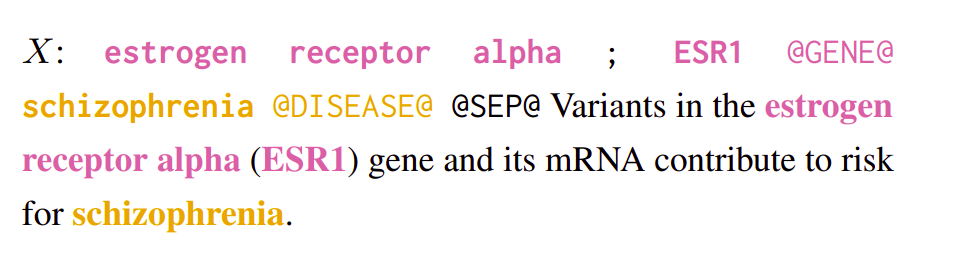
\includegraphics[width=0.7\textwidth,height=0.7\textheight,keepaspectratio]{entity_hint} 
          \end{figure}

          Full schema:

          \begin{adjustbox}{varwidth=\linewidth}%,scale=0.7}
            %% \begin{framed}
            %\centering
            \small\text{$<\textit{entity mention}_{1,1}>$ ; ... ; $<\textit{entity mention}_{1,n}>$ $@<\textit{entity type}_1 @> \dots$}

            
            \small\text{$<\textit{entity mention}_{m,1}>$ ; ... ; $<\textit{entity mention}_{m,k}>$ $@<\textit{entity type}_m @> \ldots$}
            

            \small\text{$@\text{SEP}@$ $<\textit{input text}>$}
          \end{adjustbox}



          
          Hinting is omitted for end-to-end.
        \end{frame}

        
        
        \section{Results}

        
        
        \section{Analysis}


        \begin{frame}{$n$-ary Relations (DGM)}
          \begin{figure}
            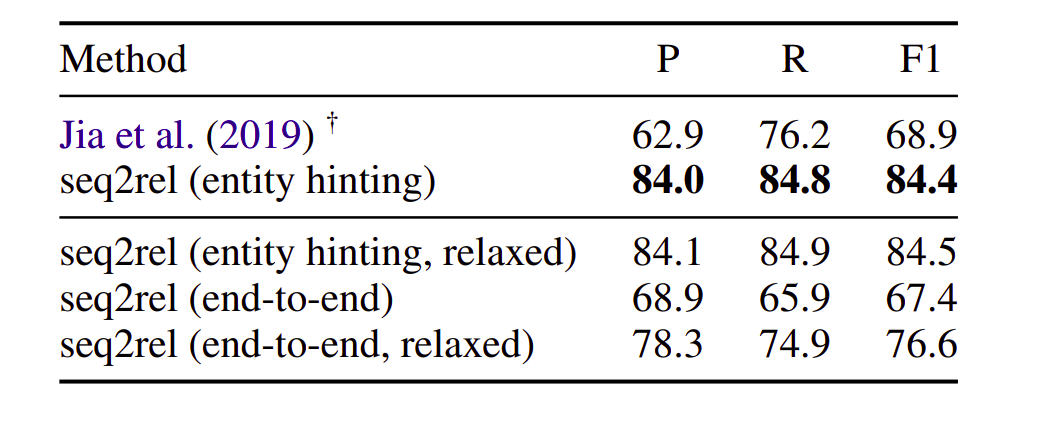
\includegraphics[width=0.7\textwidth,height=0.7\textheight,keepaspectratio]{DGM_n_ary_comparison} 
          \end{figure}
          DGM has ternary relations. Baseline, Jia et al. (2019) uses multiscale architecture
          (uses multiple representations over different sizes of text spans and types of sub-relations).
          Both use gold entities (entity hinting in seq2rel case).
        \end{frame}

        \begin{frame}{RE with Gold Entities (CDR, GDA)}
          \begin{figure}
            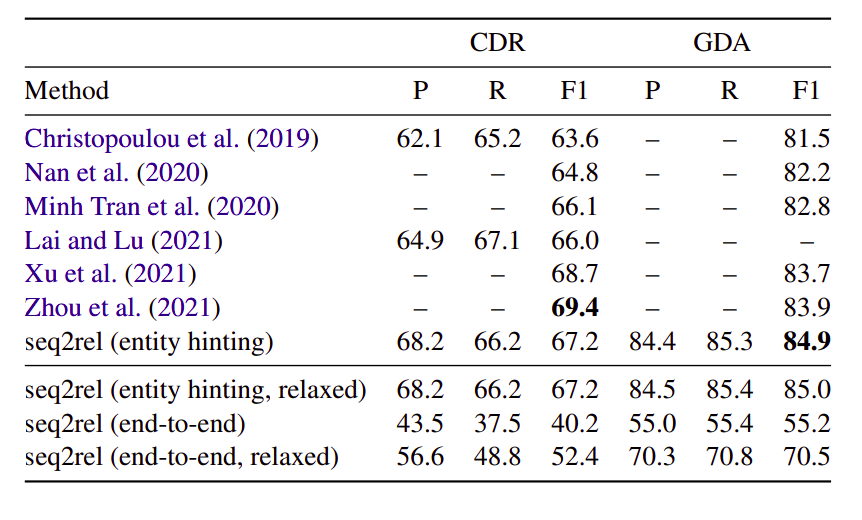
\includegraphics[width=0.7\textwidth,height=0.7\textheight,keepaspectratio]{CDR_GDA_gold_entities} 
          \end{figure}

          (Not enough room, full breakdown of baseline approaches in paper appendix {\it G})
        \end{frame}

        \begin{frame}{End-to-end RE (DocRED)}
          \begin{figure}
            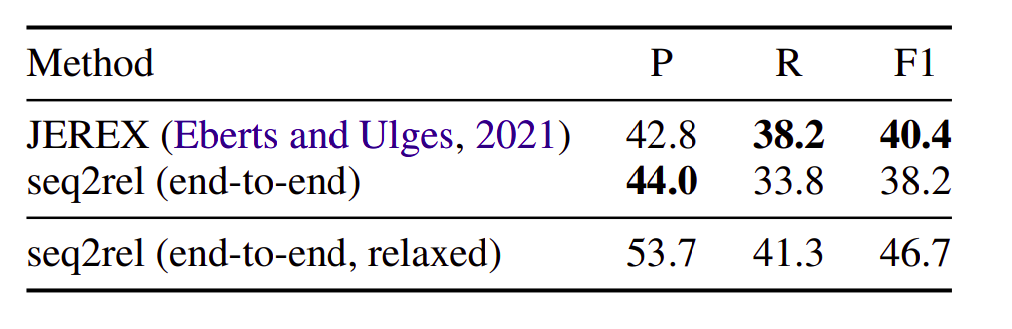
\includegraphics[width=0.7\textwidth,height=0.7\textheight,keepaspectratio]{DocRED_e2e_comparison} 
          \end{figure}
        \end{frame}

        \begin{frame}{End-to-end RE (DocRED)}          
          JEREX =  BERT with four joint task-specific
          FFNN-based components in the following order:
          \begin{itemize}
          \item
            entity mention localization,
          \item
            coreference
            resolution
          \item
            entity classification
          \item relation
            classification.
          \end{itemize}
          Two versions of
          the relation classifier, “global relation classifier” (GRC) and “multi-instance
          relation classifier” (MRC). The authors compare against
          JEREX-MRC for DocRED end to end.

        \end{frame}

        \begin{frame}{End-to-end RE Ablation (CDR, DocRED)}
          \begin{figure}
            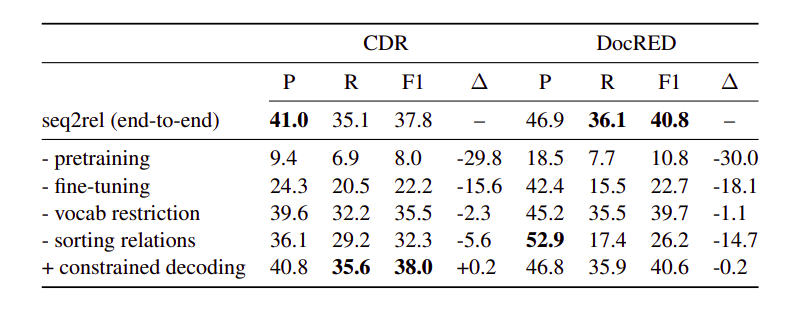
\includegraphics[width=0.7\textwidth,height=0.4\textheight,keepaspectratio]{ablation} 
          \end{figure}
          \begin{itemize}
          \item
            Fine-tuning here is wrt the encoder.
          \item
            Vocab restriction = special tokens + copy mechanism.
          \item
            Sorting relations = sorting relations by order of appearance for consistent decoding order.
          \item
            Constrained decoding = prevention of syntactically invalid output strings.
          \end{itemize}
        \end{frame}

        \begin{frame}{Training Set Size vs. Performance (CDR, GDA)}
          \begin{figure}
            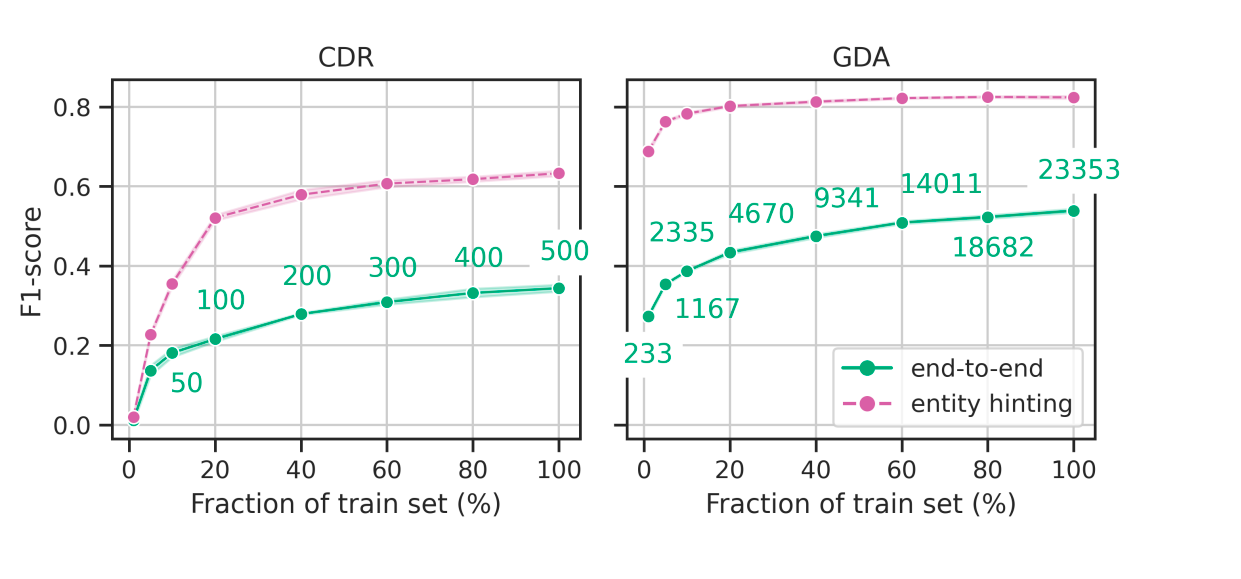
\includegraphics[width=0.7\textwidth,height=0.7\textheight,keepaspectratio]{training_set_size_plateau} 
          \end{figure}

          Due to logarithmic shape of e2e f1 against train set size authors believe e2e has potential for better scores (vs. asymptotic curves with entity hinting).
        \end{frame}

        \begin{frame}{Hyperparameter Tuning}
          \begin{figure}
            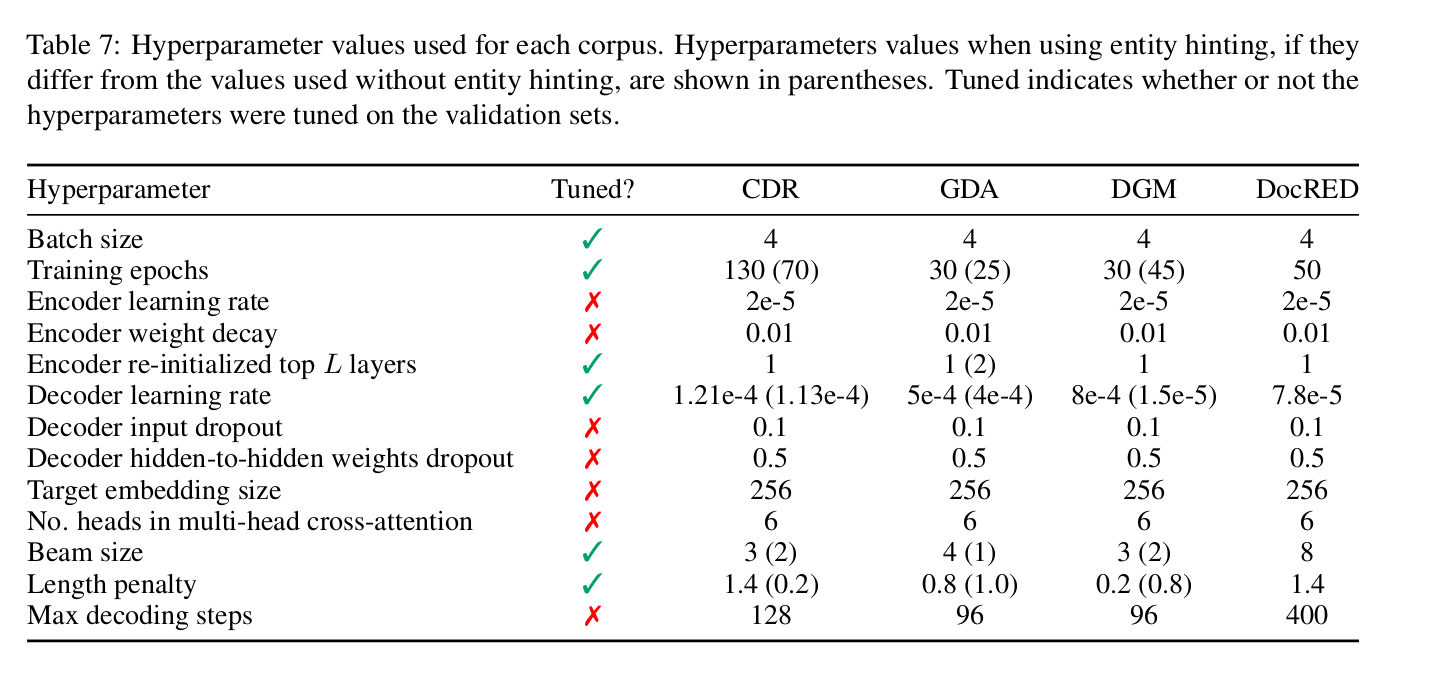
\includegraphics[width=1.0\textwidth,height=1.0\textheight,keepaspectratio]{hyperparameters} 
          \end{figure}
        \end{frame}
        
        \section{Conclusion}

        \begin{frame}{Strengths}
          Pure RE (with gold entity hinting)
          \begin{itemize}
          \item
            SOTA on GDA.
          \item
            Highly competitive on CDR.
          \item
            Markedly simpler architecure than the baselines
            \footnote{Most construct
            a document-level graph using dependency parsing,
            heuristics, or structured attention and then update
            node and edge representations using propagation.
            Xu et al. 2021 and Zhou et al. 2021 make modifications
            to transformer architecure and BERT achitecture respectively}.  
          \end{itemize}
          End-to-end
          \begin{itemize}
          \item
            Competitive result against SOTA JEREX.
          \item
            Simpler architecture than JEREX.
          \end{itemize}
          Linearization schema is easy to interpret.
          Can handle discontinuous/disjoint and nested entities.
        \end{frame}

        \begin{frame}{Limitations}
          Training strategy:
          \begin{itemize}
          \item
            Rationale not fully explained.
          \item
            Could use variation in lr scheduling\footnote{Some RT NER models rescued by cosine lr schedule} and other hyperparameters.
          \item
            Additional LSTM directionality and layering variation.
          \item
            Cross-attention mechanism variation.
          \item
            Teacher forcing, while common for seq2seq,
            gives faster convergence but possibly lower performance at inference due to exposure bias.  
          \end{itemize}
        \end{frame}

        \begin{frame}{Limitations}
          Model structure:
          \begin{itemize}
          \item
            512 token limitation.
          \item
            Bevy of architectures (especially transformer-based) for long document processing
            \footnote{E.g. Tim and Angus have extensive experience with Hierarchical Transformers
            \url{https://arxiv.org/abs/2110.13711}}  
          
            
          \end{itemize}
          Linearization schema:
          \begin{itemize}
          \item
            Ideally want order invariant scoring.
          \item
            Will this generalize to long documents with frequent correferents?
          \item
            $n>3$-ary relations?
          \end{itemize}
        \end{frame}
        
        
        \begin{frame}{Conclusion}
          \begin{itemize}
          \item
            Novel application of relatively well understood technique for an increasingly relevant task, esp. for clinicald documents.
          \item
            Many possible variations of architecture and application.
          \item
            Possible to test features/methods from baselines\footnote{dependency parses, document graphs}
            within this architecture.
          \item
            Implementation and behavior tracking easier than competition.
          \item
            More efficient than a lot of pipeline models\footnote{E.g. at least one LPLM for NER, at least one for RE}.
          \end{itemize}

          Full bibliography in paper.
        \end{frame}

        \begin{frame}{Other Helpful Links}
          \begin{itemize}
          \item
            Seq2seq:

            
            {\footnotesize \url{https://d2l.ai/chapter_recurrent-modern/seq2seq.html\#sec-seq2seq}}
          \item
            Beam search:

            
            {\small \url{https://d2l.ai/chapter_recurrent-modern/beam-search.html}}
            
          \end{itemize}
        \end{frame}
      \end{document}
      
      
